% ==============================================================================
% Topic 01: Circuit Theory Fundamentals
% Course: BE5B31ZEO
% GRADE: D | PRIORITY: [CAUTION]
% ==============================================================================

\section{Circuit Theory Fundamentals | 电路理论基础}

\begin{warnbox}[\textcolor{orange}{\textbf{[CAUTION]}} GRADE D: FOCUS MODE / 成绩D:专注模式]
\textbf{[CN]} ZEO成绩是 \textbf{D}。重点练习 KVL/KCL 计算,\textbf{关联论文}:传感器接口电路!\\
\textbf{[EN]} ZEO grade is \textbf{D}. Practice KVL/KCL calculations. \textbf{Bridge to Thesis}: Sensor interface circuits!\\
\textbf{Thesis Link}: 分压器设计 → ADC输入范围匹配 (0-3.3V for ESP32)
\end{warnbox}

\begin{defbox}{Core Survival Strategy | 核心生存策略}
\textbf{[CN]} 电路理论是电子工程的基础,但考试时间有限。本章聚焦最高频考点:\\
\textbf{[EN]} Circuit theory is EE foundation. Focus on highest-frequency exam topics:
\begin{enumerate}
    \item \textbf{[CN]} 欧姆定律 (Ohm's Law) --- 必考计算 / \textbf{[EN]} Ohm's Law --- must-know calculation
    \item \textbf{[CN]} KVL/KCL --- 电路分析核心 / \textbf{[EN]} KVL/KCL --- circuit analysis core
    \item \textbf{[CN]} 分压器 (Voltage Divider) --- 传感器接口必备 / \textbf{[EN]} Voltage Divider --- sensor interface essential
    \item \textbf{[CN]} 戴维南等效 (Thevenin) --- 简化复杂电路 / \textbf{[EN]} Thevenin --- simplify complex circuits
    \item \textbf{[CN]} 功率计算 (Power) --- 电源设计基础 / \textbf{[EN]} Power --- power supply design basis
\end{enumerate}
\tcblower
\textbf{[EN] Full Mirror}: Circuit theory survival checklist: Ohm's Law (V=IR), Kirchhoff's Laws (KVL/KCL), Voltage Divider, Thevenin Equivalent, and Power calculations.
\end{defbox}

% ------------------------------------------------------------------------------
\subsection{Ohm's Law | 欧姆定律}
% ------------------------------------------------------------------------------

\begin{formulabox}{Ohm's Law | 欧姆定律公式}
\begin{equation}
    V = I \cdot R \quad \Leftrightarrow \quad I = \frac{V}{R} \quad \Leftrightarrow \quad R = \frac{V}{I}
\end{equation}
\begin{itemize}
    \item $V$ --- 电压 (Voltage), 单位: 伏特 (V)
    \item $I$ --- 电流 (Current), 单位: 安培 (A)
    \item $R$ --- 电阻 (Resistance), 单位: 欧姆 ($\Omega$)
\end{itemize}
\tcblower
Ohm's Law: The voltage across a resistor equals current times resistance.
\end{formulabox}

\begin{studybox}{Blackboard Challenge 1: Ohm's Law | 欧姆定律计算}
\textbf{[CN] Problem / 题目:} ESP32的GPIO输出3.3V,驱动一个LED(正向压降2V),需要10mA电流。求限流电阻值。\\
\textbf{[EN] Problem:} ESP32 GPIO outputs 3.3V, driving an LED (forward drop 2V), needs 10mA. Find the limiting resistor.

\textbf{Step-by-step Solution / 分步解答}:
\begin{enumerate}
    \item \textbf{[CN]} 确定电阻两端电压 / \textbf{[EN]} Find voltage across resistor:\\ $V_R = V_{GPIO} - V_{LED} = 3.3V - 2V = 1.3V$
    \item \textbf{[CN]} 应用欧姆定律 / \textbf{[EN]} Apply Ohm's Law:\\ $R = \frac{V_R}{I} = \frac{1.3V}{10mA} = \frac{1.3V}{0.01A}$
    \item \textbf{[CN]} 计算结果 / \textbf{[EN]} Calculate result:\\ $R = 130\Omega$
\end{enumerate}
\tcblower
\textbf{Answer / 答案:} $\boxed{R = 130\Omega}$\\
\textbf{[CN]} 实际选用标准值 $150\Omega$ / \textbf{[EN]} Use standard value $150\Omega$ in practice
\end{studybox}

\begin{warnbox}{Mnemonic: VIR Triangle | 记忆口诀}
\textbf{口诀: ``伏安欧,上下分''}
\begin{center}
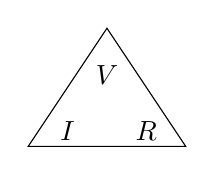
\begin{tikzpicture}
    \draw (0,0) -- (2,0) -- (1,1.5) -- cycle;
    \node at (1,0.9) {$V$};
    \node at (0.5,0.2) {$I$};
    \node at (1.5,0.2) {$R$};
\end{tikzpicture}
\end{center}
遮住要求的量,剩下的就是公式:遮V得IR,遮I得V/R,遮R得V/I
\tcblower
Cover what you want to find: Cover V $\rightarrow$ IR, Cover I $\rightarrow$ V/R, Cover R $\rightarrow$ V/I
\end{warnbox}

% ------------------------------------------------------------------------------
\subsection{Kirchhoff's Laws | 基尔霍夫定律}
% ------------------------------------------------------------------------------

\begin{formulabox}{KVL: Kirchhoff's Voltage Law | 基尔霍夫电压定律}
\begin{equation}
    \sum_{k=1}^{n} V_k = 0 \quad \text{(沿闭合回路)}
\end{equation}
\textbf{物理意义:} 沿任意闭合回路,电压升等于电压降(能量守恒)
\tcblower
KVL: The algebraic sum of voltages around any closed loop equals zero.
\end{formulabox}

\begin{formulabox}{KCL: Kirchhoff's Current Law | 基尔霍夫电流定律}
\begin{equation}
    \sum_{k=1}^{n} I_{in} = \sum_{k=1}^{m} I_{out} \quad \text{(在任意节点)}
\end{equation}
\textbf{物理意义:} 流入节点的电流等于流出节点的电流(电荷守恒)
\tcblower
KCL: The sum of currents entering a node equals the sum of currents leaving.
\end{formulabox}

\begin{studybox}{Blackboard Challenge 2: KVL Application | KVL应用}
\textbf{[CN] Problem / 题目:} 串联电路中,$V_s = 12V$,$R_1 = 2k\Omega$,$R_2 = 4k\Omega$。求各电阻上的电压。\\
\textbf{[EN] Problem:} Series circuit with $V_s = 12V$, $R_1 = 2k\Omega$, $R_2 = 4k\Omega$. Find voltage across each resistor.

\textbf{Step-by-step Solution / 分步解答}:
\begin{enumerate}
    \item \textbf{[CN]} 求总电阻 / \textbf{[EN]} Find total resistance:\\ $R_{total} = R_1 + R_2 = 2k + 4k = 6k\Omega$
    \item \textbf{[CN]} 求电流 / \textbf{[EN]} Find current:\\ $I = \frac{V_s}{R_{total}} = \frac{12V}{6k\Omega} = 2mA$
    \item \textbf{[CN]} 求$V_{R1}$ / \textbf{[EN]} Find $V_{R1}$:\\ $V_{R1} = I \cdot R_1 = 2mA \times 2k\Omega = 4V$
    \item \textbf{[CN]} 求$V_{R2}$ / \textbf{[EN]} Find $V_{R2}$:\\ $V_{R2} = I \cdot R_2 = 2mA \times 4k\Omega = 8V$
    \item \textbf{[CN]} 验证KVL / \textbf{[EN]} Verify KVL:\\ $V_s - V_{R1} - V_{R2} = 12 - 4 - 8 = 0$ \checkmark
\end{enumerate}
\tcblower
\textbf{Answer / 答案:} $\boxed{V_{R1} = 4V, \quad V_{R2} = 8V}$
\end{studybox}

\begin{warnbox}{Mnemonic: KVL/KCL | 记忆口诀}
\textbf{口诀: ``电压绕圈零,电流进出平''}
\begin{itemize}
    \item KVL: 电压绕圈(Loop)加起来等于零
    \item KCL: 电流进出节点(Node)要平衡
\end{itemize}
\tcblower
KVL: Voltages around Loop = 0; KCL: Currents at Node balance out.
\end{warnbox}

% ------------------------------------------------------------------------------
\subsection{Voltage Divider | 分压器}
% ------------------------------------------------------------------------------

\begin{formulabox}{Voltage Divider Formula | 分压公式}
\begin{equation}
    V_{out} = V_{in} \cdot \frac{R_2}{R_1 + R_2}
\end{equation}
\begin{center}
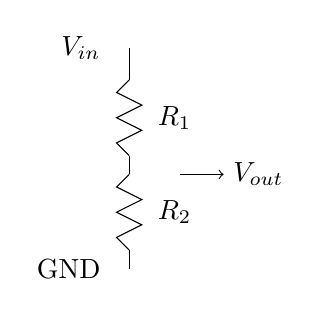
\begin{tikzpicture}[scale=0.8]
    \draw (0,3) -- (0,2.5);
    \draw (0,2.5) -- (-0.2,2.3) -- (0.2,2.1) -- (-0.2,1.9) -- (0.2,1.7) -- (-0.2,1.5) -- (0,1.3);
    \node[right] at (0.3,1.9) {$R_1$};
    \draw (0,1.3) -- (0,1);
    \draw (0,1) -- (-0.2,0.8) -- (0.2,0.6) -- (-0.2,0.4) -- (0.2,0.2) -- (-0.2,0) -- (0,-0.2);
    \node[right] at (0.3,0.4) {$R_2$};
    \draw (0,-0.2) -- (0,-0.5);
    \node[left] at (-0.3,3) {$V_{in}$};
    \node[left] at (-0.3,-0.5) {GND};
    \draw[->] (0.8,1) -- (1.5,1);
    \node[right] at (1.5,1) {$V_{out}$};
\end{tikzpicture}
\end{center}
\tcblower
The output voltage is proportional to the ratio of $R_2$ to total resistance.
\end{formulabox}

\begin{studybox}{Blackboard Challenge 3: Voltage Divider | 分压器计算}
\textbf{Problem:} 设计分压电路将5V传感器信号降至ESP32可接受的3.3V。

\textbf{Step-by-step Solution:}
\begin{enumerate}
    \item 分压比: $\frac{V_{out}}{V_{in}} = \frac{3.3V}{5V} = 0.66$
    \item 设$R_1 = 10k\Omega$,求$R_2$:
    \item $\frac{R_2}{R_1 + R_2} = 0.66$
    \item $R_2 = 0.66(R_1 + R_2)$
    \item $R_2 = 0.66R_1 + 0.66R_2$
    \item $0.34R_2 = 0.66R_1$
    \item $R_2 = \frac{0.66}{0.34} \times 10k = 19.4k\Omega$
\end{enumerate}
\tcblower
\textbf{Answer:} $\boxed{R_1 = 10k\Omega, \quad R_2 = 20k\Omega}$ (使用标准值)
\end{studybox}

\begin{warnbox}{Mnemonic: Voltage Divider | 记忆口诀}
\textbf{口诀: ``下分上总,电压按比分''}

分压器输出 = 输入电压 $\times$ (下面电阻 / 总电阻)

\textbf{注意:} 负载会影响分压比!带负载时$R_2$要与负载并联计算。
\tcblower
Output = Input $\times$ (Bottom R / Total R). Load affects the ratio!
\end{warnbox}

% ------------------------------------------------------------------------------
\subsection{Thevenin Equivalent | 戴维南等效电路}
% ------------------------------------------------------------------------------

\begin{formulabox}{Thevenin Theorem | 戴维南定理}
任何线性二端网络可等效为:
\begin{equation}
    V_{th} = \text{开路电压 (Open-circuit voltage)}
\end{equation}
\begin{equation}
    R_{th} = \text{从端口看入的等效电阻 (Equivalent resistance)}
\end{equation}
\begin{center}
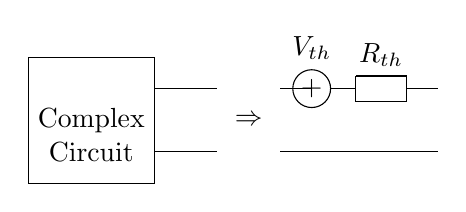
\begin{tikzpicture}[scale=0.8]
    \draw (0,0) rectangle (2,2);
    \node at (1,1) {Complex};
    \node at (1,0.5) {Circuit};
    \draw (2,1.5) -- (3,1.5);
    \draw (2,0.5) -- (3,0.5);
    \node at (3.5,1) {$\Rightarrow$};
    \draw (4,1.5) -- (4.5,1.5);
    \draw (4.5,1.5) circle (0.3);
    \node at (4.5,1.5) {$+$};
    \node[above] at (4.5,1.8) {$V_{th}$};
    \draw (4.8,1.5) -- (5.2,1.5);
    \draw (5.2,1.7) -- (5.2,1.3) -- (6,1.3) -- (6,1.7) -- (5.2,1.7);
    \node[above] at (5.6,1.7) {$R_{th}$};
    \draw (6,1.5) -- (6.5,1.5);
    \draw (4,0.5) -- (6.5,0.5);
\end{tikzpicture}
\end{center}
\tcblower
Thevenin: Any linear circuit = Voltage source $V_{th}$ + Series resistance $R_{th}$
\end{formulabox}

\begin{studybox}{Blackboard Challenge 4: Thevenin Equivalent | 戴维南等效}
\textbf{Problem:} 求下图电路的戴维南等效电路(从AB端口看)。
$V_s = 10V$, $R_1 = 2\Omega$, $R_2 = 3\Omega$

\textbf{Step-by-step Solution:}
\begin{enumerate}
    \item \textbf{求$V_{th}$(开路电压):}
    \begin{itemize}
        \item AB开路时,$R_2$无电流
        \item $V_{th} = V_s \cdot \frac{R_2}{R_1 + R_2} = 10 \cdot \frac{3}{5} = 6V$
    \end{itemize}
    \item \textbf{求$R_{th}$(等效电阻):}
    \begin{itemize}
        \item 将电压源短路(理想电压源内阻为0)
        \item $R_{th} = R_1 \parallel R_2 = \frac{R_1 \cdot R_2}{R_1 + R_2} = \frac{2 \times 3}{5} = 1.2\Omega$
    \end{itemize}
\end{enumerate}
\tcblower
\textbf{Answer:} $\boxed{V_{th} = 6V, \quad R_{th} = 1.2\Omega}$
\end{studybox}

\begin{warnbox}{Mnemonic: Thevenin Steps | 记忆口诀}
\textbf{口诀: ``开路求压,短源求阻''}
\begin{enumerate}
    \item 开路求压: 断开负载,计算开路电压$V_{th}$
    \item 短源求阻: 电压源短路,电流源开路,计算等效电阻$R_{th}$
\end{enumerate}
\tcblower
Open for $V_{th}$, Short sources for $R_{th}$
\end{warnbox}

% ------------------------------------------------------------------------------
\subsection{Transformer | 变压器}
% ------------------------------------------------------------------------------

\begin{formulabox}{Transformer Equations | 变压器公式}
\textbf{匝数比 (Turns Ratio):}
\begin{equation}
    \frac{V_1}{V_2} = \frac{N_1}{N_2} = n \quad \text{(电压比等于匝数比)}
\end{equation}
\begin{equation}
    \frac{I_1}{I_2} = \frac{N_2}{N_1} = \frac{1}{n} \quad \text{(电流比等于匝数比的倒数)}
\end{equation}
\textbf{功率关系 (理想变压器):}
\begin{equation}
    P_1 = P_2 \quad \Rightarrow \quad V_1 I_1 = V_2 I_2
\end{equation}
\textbf{阻抗变换:}
\begin{equation}
    Z_1 = n^2 \cdot Z_2 \quad \text{(阻抗按匝数比平方变换)}
\end{equation}
\tcblower
Ideal transformer: Voltage ratio = Turns ratio; Current ratio = Inverse turns ratio.
\end{formulabox}

\begin{studybox}{Blackboard Challenge 5: Transformer | 变压器计算}
\textbf{Problem:} 变压器初级220V,次级需要12V供ESP32电源模块。匝数比和次级电流(初级0.1A)?

\textbf{Step-by-step Solution:}
\begin{enumerate}
    \item 匝数比: $n = \frac{N_1}{N_2} = \frac{V_1}{V_2} = \frac{220V}{12V} = 18.33$
    \item 电流关系: $I_2 = I_1 \cdot n = 0.1A \times 18.33 = 1.833A$
    \item 验证功率: $P_1 = 220 \times 0.1 = 22W$, $P_2 = 12 \times 1.833 = 22W$ \checkmark
\end{enumerate}
\tcblower
\textbf{Answer:} $\boxed{n \approx 18:1, \quad I_2 \approx 1.83A}$
\end{studybox}

% ------------------------------------------------------------------------------
\subsection{AC Power | 交流功率}
% ------------------------------------------------------------------------------

\begin{formulabox}{AC Power Triangle | 交流功率三角形}
\begin{equation}
    S = V \cdot I = \sqrt{P^2 + Q^2} \quad \text{(视在功率 Apparent Power, VA)}
\end{equation}
\begin{equation}
    P = V \cdot I \cdot \cos\phi \quad \text{(有功功率 Active Power, W)}
\end{equation}
\begin{equation}
    Q = V \cdot I \cdot \sin\phi \quad \text{(无功功率 Reactive Power, VAR)}
\end{equation}
\begin{equation}
    \text{Power Factor: } PF = \cos\phi = \frac{P}{S}
\end{equation}
\tcblower
Power triangle: $S^2 = P^2 + Q^2$, Power Factor = $\cos\phi$ = P/S
\end{formulabox}

\begin{studybox}{Blackboard Challenge 6: Power Factor | 功率因数计算}
\textbf{Problem:} 电机额定220V,电流5A,功率因数0.8(滞后)。求P、Q、S。

\textbf{Step-by-step Solution:}
\begin{enumerate}
    \item 视在功率: $S = V \cdot I = 220 \times 5 = 1100VA$
    \item 有功功率: $P = S \cdot \cos\phi = 1100 \times 0.8 = 880W$
    \item 无功功率: $Q = S \cdot \sin\phi = 1100 \times 0.6 = 660VAR$
    \item 验证: $\sqrt{880^2 + 660^2} = \sqrt{774400 + 435600} = 1100VA$ \checkmark
\end{enumerate}
\tcblower
\textbf{Answer:} $\boxed{S = 1100VA, \quad P = 880W, \quad Q = 660VAR}$
\end{studybox}

\begin{warnbox}{Mnemonic: Power Triangle | 记忆口诀}
\textbf{口诀: ``视在为斜,有功为底,无功为高''}
\begin{center}
\begin{tikzpicture}[scale=0.6]
    \draw[thick] (0,0) -- (4,0) node[midway,below] {P (有功)};
    \draw[thick] (4,0) -- (4,3) node[midway,right] {Q (无功)};
    \draw[thick] (0,0) -- (4,3) node[midway,above left] {S (视在)};
    \draw (0.8,0) arc (0:36.87:0.8);
    \node at (1.2,0.3) {$\phi$};
\end{tikzpicture}
\end{center}
\textbf{功率因数低的危害:} 电流大但做功少,浪费电网容量
\tcblower
Power triangle: S (hypotenuse), P (adjacent), Q (opposite), angle $\phi$
\end{warnbox}

% ------------------------------------------------------------------------------
\subsection{Thesis Application: ESP32 Power Supply | 论文应用}
% ------------------------------------------------------------------------------

\begin{thesisbox}{ESP32 IoT Sensor Power Design | ESP32物联网传感器电源设计}
\textbf{论文关联:} 智能家居传感器节点的电源系统设计

\textbf{实际应用:}
\begin{enumerate}
    \item \textbf{电源模块选择:}
    \begin{itemize}
        \item ESP32工作电压: 3.0--3.6V(典型3.3V)
        \item 峰值电流: WiFi发射时可达500mA
        \item 选用AMS1117-3.3 LDO或MP1584 DC-DC
    \end{itemize}
    
    \item \textbf{分压器应用:}
    \begin{itemize}
        \item 电池电压监测: 锂电池4.2V $\rightarrow$ ADC可测范围
        \item $V_{out} = 4.2V \times \frac{100k}{100k+100k} = 2.1V$
    \end{itemize}
    
    \item \textbf{功耗计算:}
    \begin{itemize}
        \item Deep Sleep: 10$\mu$A
        \item Active: 80mA
        \item WiFi TX: 380mA
        \item 平均功耗决定电池寿命
    \end{itemize}
\end{enumerate}
\tcblower
\textbf{Thesis Link:} Power supply design for IoT sensor nodes using voltage dividers for battery monitoring and proper regulator selection for ESP32's varying current demands.
\end{thesisbox}

% ------------------------------------------------------------------------------
\subsection{USB Cable Voltage Drop | USB线缆压降 (Thesis Critical!)}
% ------------------------------------------------------------------------------

\begin{studybox}{Blackboard Challenge 7: USB Cable Voltage Drop | USB线缆压降}
\textbf{[CN] 场景}: 「你的ESP32通过2米USB线供电,WiFi发射时电流500mA。USB线电阻0.5$\Omega$(往返)。求到达ESP32的电压。」

\textbf{Problem:} 5V USB电源经过有电阻的线缆,电压会下降

\textbf{Step-by-step Solution:}
\begin{enumerate}
    \item 计算线缆压降: $V_{drop} = I \times R_{cable} = 0.5A \times 0.5\Omega = 0.25V$
    \item 到达ESP32的电压: $V_{ESP32} = V_{USB} - V_{drop} = 5V - 0.25V = 4.75V$
    \item 经过LDO后: $V_{out} = 3.3V$(LDO只要输入>4V就能稳定输出3.3V)
\end{enumerate}

\textbf{危险情况}:
\begin{itemize}
    \item 如果线缆更长(5m)或更细(AWG28), $R_{cable}$可能达到2$\Omega$
    \item 压降: $0.5A \times 2\Omega = 1V$, 到达电压只有4V
    \item 接近LDO的dropout voltage极限!
\end{itemize}

\tcblower
\textbf{Answer:} $\boxed{V_{ESP32} = 4.75V}$ (OK),但长/细线缆可能导致电压过低
\end{studybox}

\begin{thesisbox}{Thesis Bridge: Real-World Power Issues | 实际电源问题}
\textbf{[CN]}: 这是我在开发中遇到的真实问题...

\textbf{Script}: ``During my thesis development, I experienced random ESP32 resets. Investigation revealed:
\begin{itemize}
    \item \textbf{Root cause}: Cheap USB cable with high resistance
    \item \textbf{Symptom}: WiFi TX (500mA) caused voltage sag below 3.0V
    \item \textbf{Solution}: 
    \begin{enumerate}
        \item Replaced with quality cable (AWG24, shorter)
        \item Added 470$\mu$F bulk capacitor near ESP32
        \item Capacitor provides charge during current spikes
    \end{enumerate}
\end{itemize}

The capacitor calculation:
\[
V_{sag} = \frac{I \cdot \Delta t}{C} = \frac{0.5A \times 0.001s}{470\mu F} = 1.06V
\]

With proper capacitor, voltage sag is limited even during WiFi bursts.''
\end{thesisbox}

% ------------------------------------------------------------------------------
\subsection{Battery Life Calculation | 电池寿命计算}
% ------------------------------------------------------------------------------

\begin{studybox}{Blackboard Challenge 8: Battery Life | 电池续航计算}
\textbf{[CN] 场景}: 「ESP32用2000mAh锂电池供电,每5分钟测量一次并上传数据。求电池寿命。」

\textbf{功耗模式}:
\begin{itemize}
    \item Deep Sleep: $I_{sleep} = 10\mu A$, $t_{sleep} = 299s$
    \item Active + WiFi: $I_{active} = 150mA$ (average), $t_{active} = 1s$
\end{itemize}

\textbf{Step-by-step Solution:}
\begin{enumerate}
    \item 每周期消耗电量:
    \begin{align}
        Q_{cycle} &= I_{sleep} \times t_{sleep} + I_{active} \times t_{active} \\
        &= 10\mu A \times 299s + 150mA \times 1s \\
        &= 2.99mAs + 150mAs = 152.99mAs
    \end{align}
    
    \item 每周期时间: $T_{cycle} = 300s = 5min$
    
    \item 平均电流:
    \[
    I_{avg} = \frac{Q_{cycle}}{T_{cycle}} = \frac{152.99mAs}{300s} = 0.51mA
    \]
    
    \item 电池寿命:
    \[
    t_{life} = \frac{C_{battery}}{I_{avg}} = \frac{2000mAh}{0.51mA} = 3922h \approx \boxed{163 \text{ days}}
    \]
\end{enumerate}

\tcblower
\textbf{Answer:} 约163天,实际会因自放电和效率损失约减少20\%
\end{studybox}

\begin{thesisbox}{Thesis Bridge: Power Optimization | 功耗优化}
\textbf{[CN]}: 这是我论文中的功耗优化策略...

\textbf{Script}: ``To maximize battery life in my IoT sensor:
\begin{enumerate}
    \item \textbf{Deep Sleep}: ESP32 consumes only 10$\mu$A (vs 80mA active)
    \item \textbf{Batch Uploads}: Collect multiple readings, send once
    \item \textbf{WiFi Fast Connect}: Store last AP credentials, skip scan
    \item \textbf{Duty Cycling}: 5-minute interval is good balance
\end{enumerate}

\textbf{Power budget breakdown}:
\begin{center}
\begin{tabular}{|l|c|c|}
\hline
\textbf{State} & \textbf{Current} & \textbf{Time/Cycle} \\
\hline
Deep Sleep & 10$\mu$A & 299s (99.67\%) \\
Wake + Measure & 80mA & 0.5s \\
WiFi Connect & 120mA & 0.3s \\
WiFi TX & 200mA & 0.2s \\
\hline
\textbf{Average} & \textbf{0.51mA} & \\
\hline
\end{tabular}
\end{center}

The key insight: 99.67\% of time in deep sleep dominates the power budget.''
\end{thesisbox}

% ------------------------------------------------------------------------------
\subsection{Capacitor Sizing | 电容选型}
% ------------------------------------------------------------------------------

\begin{studybox}{Blackboard Challenge 9: Decoupling Capacitor | 去耦电容}
\textbf{[CN] 场景}: 「ESP32电源需要平滑。选择合适的去耦电容组合。」

\textbf{Design Approach / 设计方法}:

\textbf{1. Bulk Capacitor (储能)}:
\begin{itemize}
    \item 目的: 提供瞬态电流
    \item 公式: $C = \frac{I \cdot \Delta t}{\Delta V}$
    \item 例: $C = \frac{0.5A \times 0.001s}{0.1V} = 5000\mu F$
    \item 实际选用: $470\mu F$ 电解 + $10\mu F$ 陶瓷
\end{itemize}

\textbf{2. High-Frequency Decoupling (高频去耦)}:
\begin{itemize}
    \item 目的: 抑制高频噪声
    \item 选择: $100nF$ 陶瓷电容(靠近芯片引脚)
    \item 自谐振频率: $f_r = \frac{1}{2\pi\sqrt{LC}}$
\end{itemize}

\textbf{Complete Power Rail}:
\[
\text{5V} \rightarrow 470\mu F \rightarrow \text{LDO} \rightarrow 10\mu F \rightarrow 100nF \rightarrow \text{ESP32}
\]

\tcblower
\textbf{[EN]}: Use multi-stage decoupling: bulk caps for energy storage, ceramic caps for high-frequency filtering.
\end{studybox}

% ------------------------------------------------------------------------------
\subsection{Quick Reference | 速查表}
% ------------------------------------------------------------------------------

\begin{formulabox}{Survival Formula Sheet | 生存公式速查}
\begin{center}
\renewcommand{\arraystretch}{1.5}
\begin{tabular}{|l|l|l|}
\hline
\textbf{概念} & \textbf{公式} & \textbf{口诀} \\
\hline
Ohm's Law & $V = IR$ & 伏安欧,上下分 \\
\hline
KVL & $\sum V = 0$ & 电压绕圈零 \\
\hline
KCL & $\sum I_{in} = \sum I_{out}$ & 电流进出平 \\
\hline
Voltage Divider & $V_{out} = V_{in} \cdot \frac{R_2}{R_1+R_2}$ & 下分上总 \\
\hline
Parallel R & $R_p = \frac{R_1 R_2}{R_1+R_2}$ & 积除和 \\
\hline
Power & $P = VI = I^2R = \frac{V^2}{R}$ & 功率三公式 \\
\hline
Transformer & $\frac{V_1}{V_2} = \frac{N_1}{N_2}$ & 压比等匝比 \\
\hline
Power Factor & $PF = \cos\phi = \frac{P}{S}$ & 有功除视在 \\
\hline
\end{tabular}
\end{center}
\tcblower
Keep this formula sheet handy for the exam. Master these 8 formulas for survival!
\end{formulabox}
